\documentclass[conference]{IEEEtran}
\usepackage{graphicx,booktabs,amsmath,url,hyperref}
\hypersetup{hidelinks}
\title{Evaluating Identifier-Preserving Hybrid Retrieval for Technical Document Search}
\author{\IEEEauthorblockN{Project Research Report}\IEEEauthorblockA{Author-Annotated Exploratory Study}}
\begin{document}
\maketitle
\begin{abstract}
This paper reports a reproducible exploratory evaluation of identifier-aware hybrid retrieval. It uses 150 source-attributed technical documents and an author-annotated CVE-only subset of 30 queries. No model is trained. The 18-query held-out result is reported with explicit annotation and coverage limitations.
\end{abstract}
\begin{IEEEkeywords}hybrid retrieval, CVE, identifiers, exploratory evaluation\end{IEEEkeywords}
\section{Introduction}
Technical queries can contain identifiers where a close variant denotes another entity. This work compares TF--IDF, pretrained MiniLM, reciprocal rank fusion (RRF), and an identifier-aware RRF adjustment. The study is exploratory: annotations originate with the project author and are not independently verified. The original independent-review protocol is preserved, but it was amended before Phase 2 ranking because the returned review material lacked independent-review provenance.

\section{Problem Formulation and Research Question}
Given a query $q$, document corpus $\mathcal{D}$, and a ranking baseline, the task is to rank source passages that directly answer $q$ while avoiding explicit same-family identifier conflicts. The exploratory research question is: on a development-selected, held-out author-annotated CVE subset, how does an explainable identifier-aware reranker compare with unchanged RRF and its lexical and dense components? The question is intentionally empirical and does not assert general effectiveness.

\section{Related Work}
Sentence-BERT provides a practical framework for sentence embeddings and cosine retrieval \cite{reimers}. RRF combines ranked lists without learning a fusion model \cite{cormack}. Sparse, dense, and hybrid retrieval have been studied extensively \cite{luan}; COIL illustrates the value of exact lexical evidence in learned retrieval \cite{gao}. BEIR emphasizes heterogeneous evaluation and caution around broad zero-shot claims \cite{beir}.

\section{Retrieval Framework}
Each document is represented by title plus text. TF--IDF uses word-level lexical retrieval. MiniLM uses the existing sentence-transformers all-MiniLM-L6-v2 model at immutable revision 1110a243fdf4706b3f48f1d95db1a4f5529b4d41, normalized CPU embeddings, and cosine ranking. Standard RRF combines the two full rankings:
\begin{equation}
 S_{\mathrm{RRF}}(d)=\sum_{L:d\in L}\frac{1}{60+r_L(d)}.
\end{equation}
The parser recognizes explicit CVE IDs and supported ESP32 variants. For identifier sets $Q$ and $D$, the adjustment is
\begin{equation}
 S(d)=S_{\mathrm{RRF}}(d)+\lambda_m\frac{|Q\cap D|}{|Q|}-\lambda_c c(q,d).
\end{equation}
\begin{figure*}[t]\centering
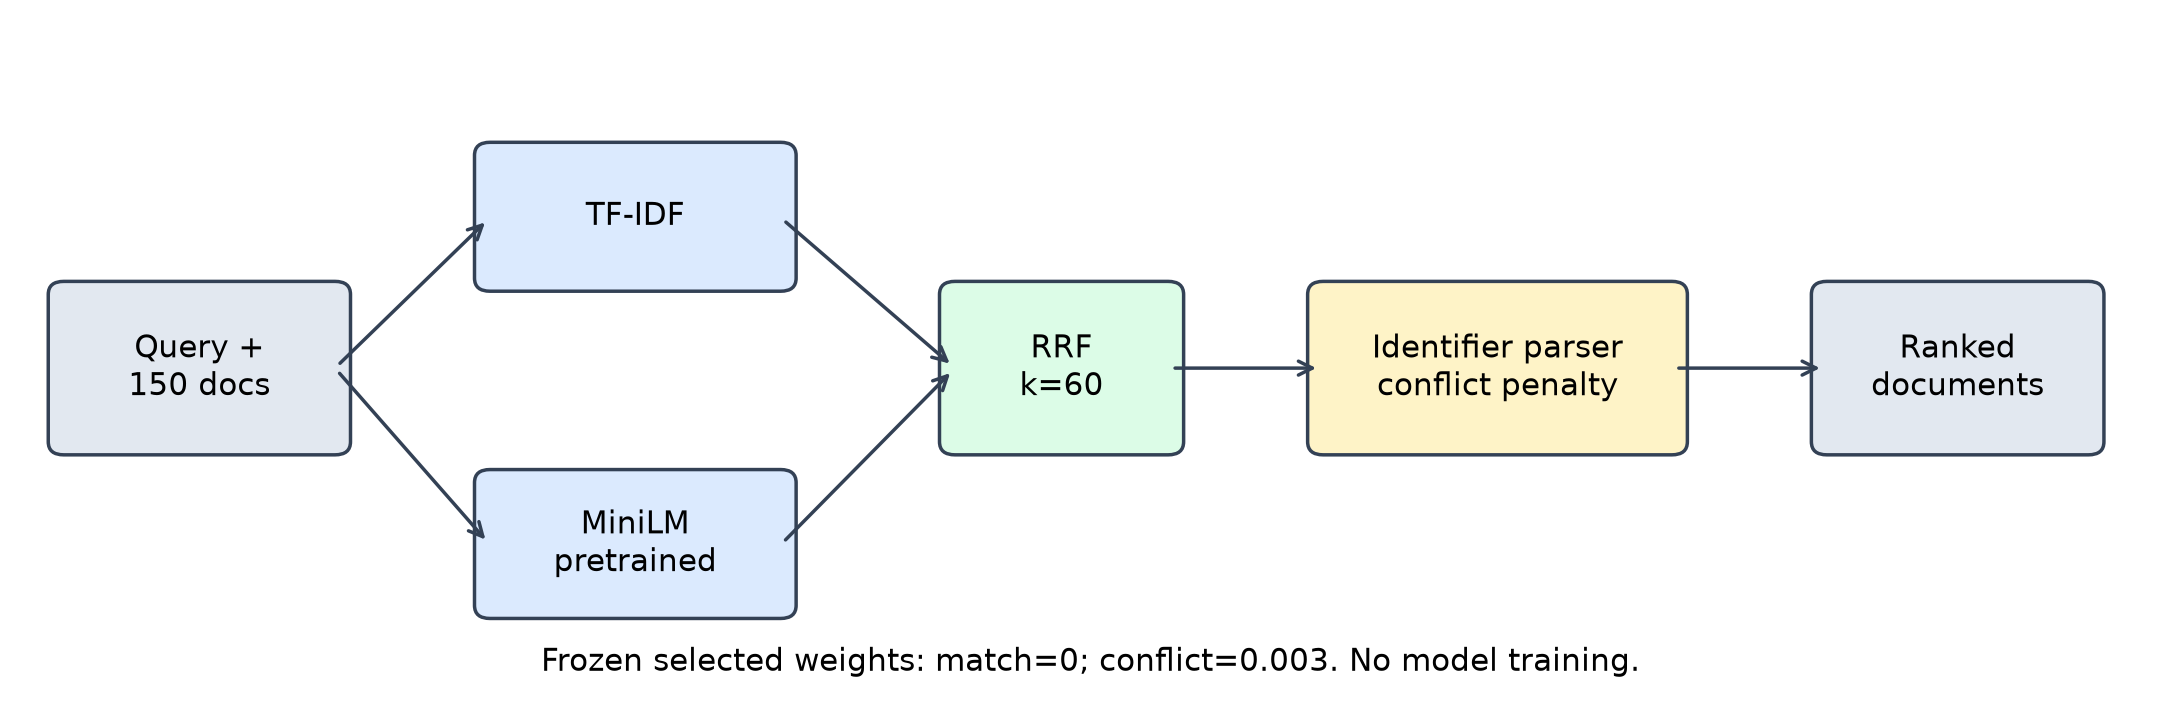
\includegraphics[width=.94\textwidth]{../../outputs/phase2/stage18/figures/retrieval_architecture.png}
\caption{Frozen Phase 2 retrieval pipeline.}\label{fig:architecture}
\end{figure*}
\section{Dataset and Eligibility}
The corpus has 150 source-attributed passages: 90 official CVE records and 60 Espressif source chunks. There are 70 question-first drafts and 273 immutable author labels: 102 relevant and 171 irrelevant. Their semantic accuracy is not independently verified.

Eligibility was determined before retrieval. An included query required author validity yes, an author-positive candidate, valid pinned provenance, and a raw source containing the requested target. For CVE records, the canonical record qualified even when its short excerpt omitted the CVE string. Seventy author-positive rows without retained target evidence became unknown only in separate derived qrels; original labels were not edited or made negative. Two target-containing CVE cross-references were retained.

\begin{figure}[t]\centering
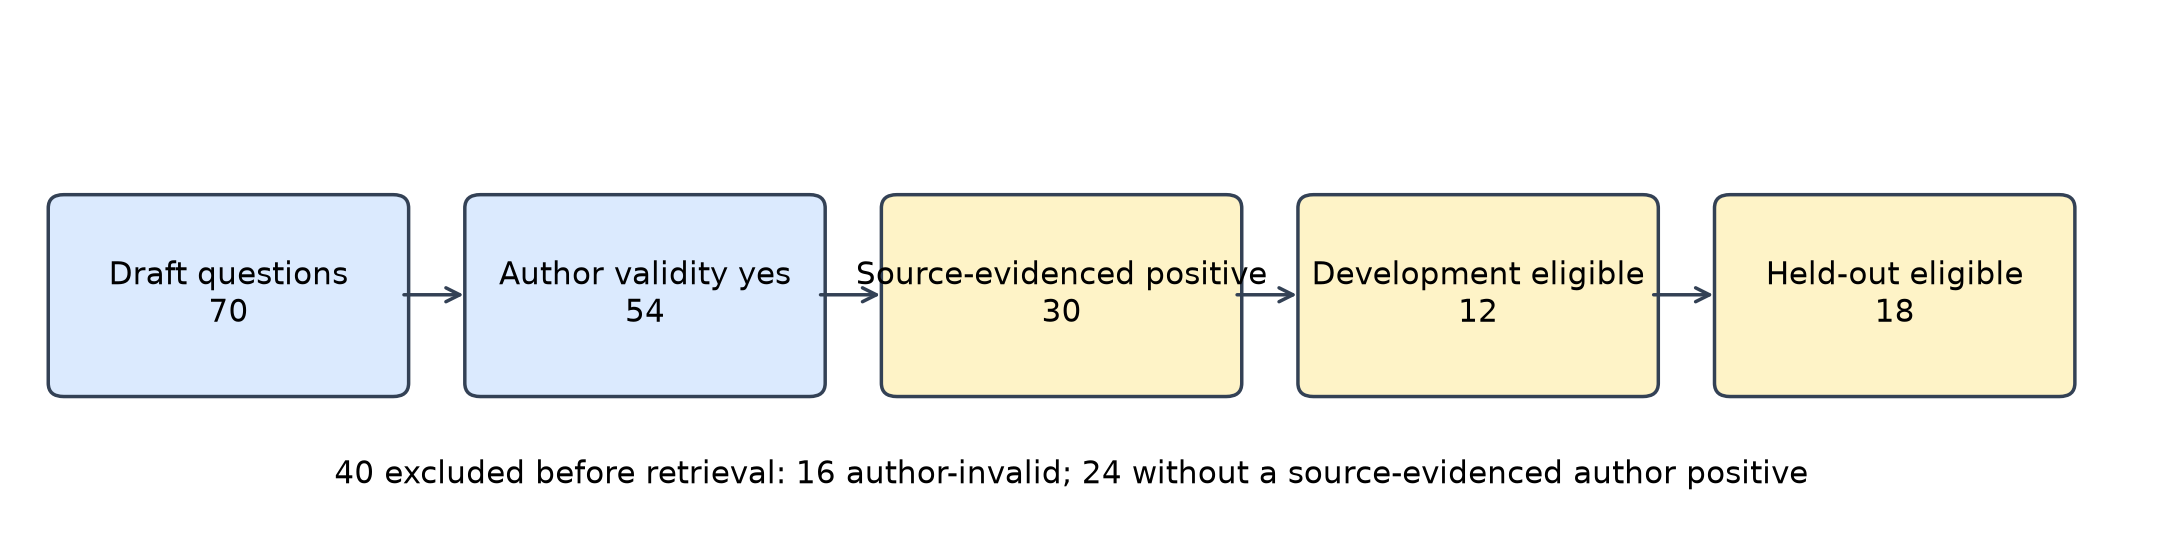
\includegraphics[width=\columnwidth]{../../outputs/phase2/stage18/figures/eligibility_flow.png}
\caption{Eligibility flow executed before Phase 2 retrieval.}\label{fig:flow}
\end{figure}

Thirty CVE queries meet this conservative policy: 12 development and 18 held-out test queries, with 32 source-evidenced positives. Forty queries are excluded before retrieval: 16 are author-invalid and 24 lack an evidence-supported author positive. The 152 additional source-backed candidates remain unjudged and are not promoted to ground truth. Thus the final subset cannot support claims about ESP32 variants or natural-language needs.

\section{Experimental Setup}
Development-only selection evaluates match weights $\{0,.003,.006,.012\}$ and conflict weights $\{0,.003,.006\}$. The lexicographic rule maximizes identifier MRR@10, minimizes the observed upper WrongIdentifier@1 bound, maximizes Recall@5, then minimizes total weight, match weight, and conflict weight. Several settings tie; the rule selects $(\lambda_m,\lambda_c)=(0,.003)$. Corpus, code, model revision, configuration, seed, and test hashes are frozen before test ranking.

For known-positive set $R$, Recall@5 is $|R\cap L_5|/|R|$, MRR@10 is the reciprocal rank of the first known positive within ten, and nDCG@10 is binary DCG normalized by ideal DCG. Unjudged pairs are unknown, not negative. WrongIdentifier@1 reports observed and upper bounds. Paired percentile bootstrap uses 10,000 resamples and seed 42.
\section{Held-out Results}
Table~\ref{tab:results} reports the 18-query held-out exploratory result. Identifier-aware reranking improves MRR@10 over RRF by .1926; its descriptive bootstrap interval is [.0556, .3481]. It has five gains, zero losses, and thirteen ties. Recall@5 does not change. This interval is not proof of statistically significant or generalizable improvement.

\begin{table}[t]\caption{Held-out exploratory results (18 CVE queries).}\label{tab:results}\centering\footnotesize
\begin{tabular}{lrrrr}\toprule
System & MRR@10 & R@5 & nDCG@10 & Wrong-ID\\\midrule
TF--IDF & .8667 & .8889 & .8844 & 0--3/18\\
MiniLM & .7278 & .8333 & .7801 & 0--7/18\\
RRF & .8074 & 1.0000 & .8544 & 0--5/18\\
Match-only & .8074 & 1.0000 & .8544 & 0--5/18\\
Identifier-aware & 1.0000 & 1.0000 & 1.0000 & 0--0/18\\\bottomrule
\end{tabular}\end{table}
\begin{figure}[t]\centering
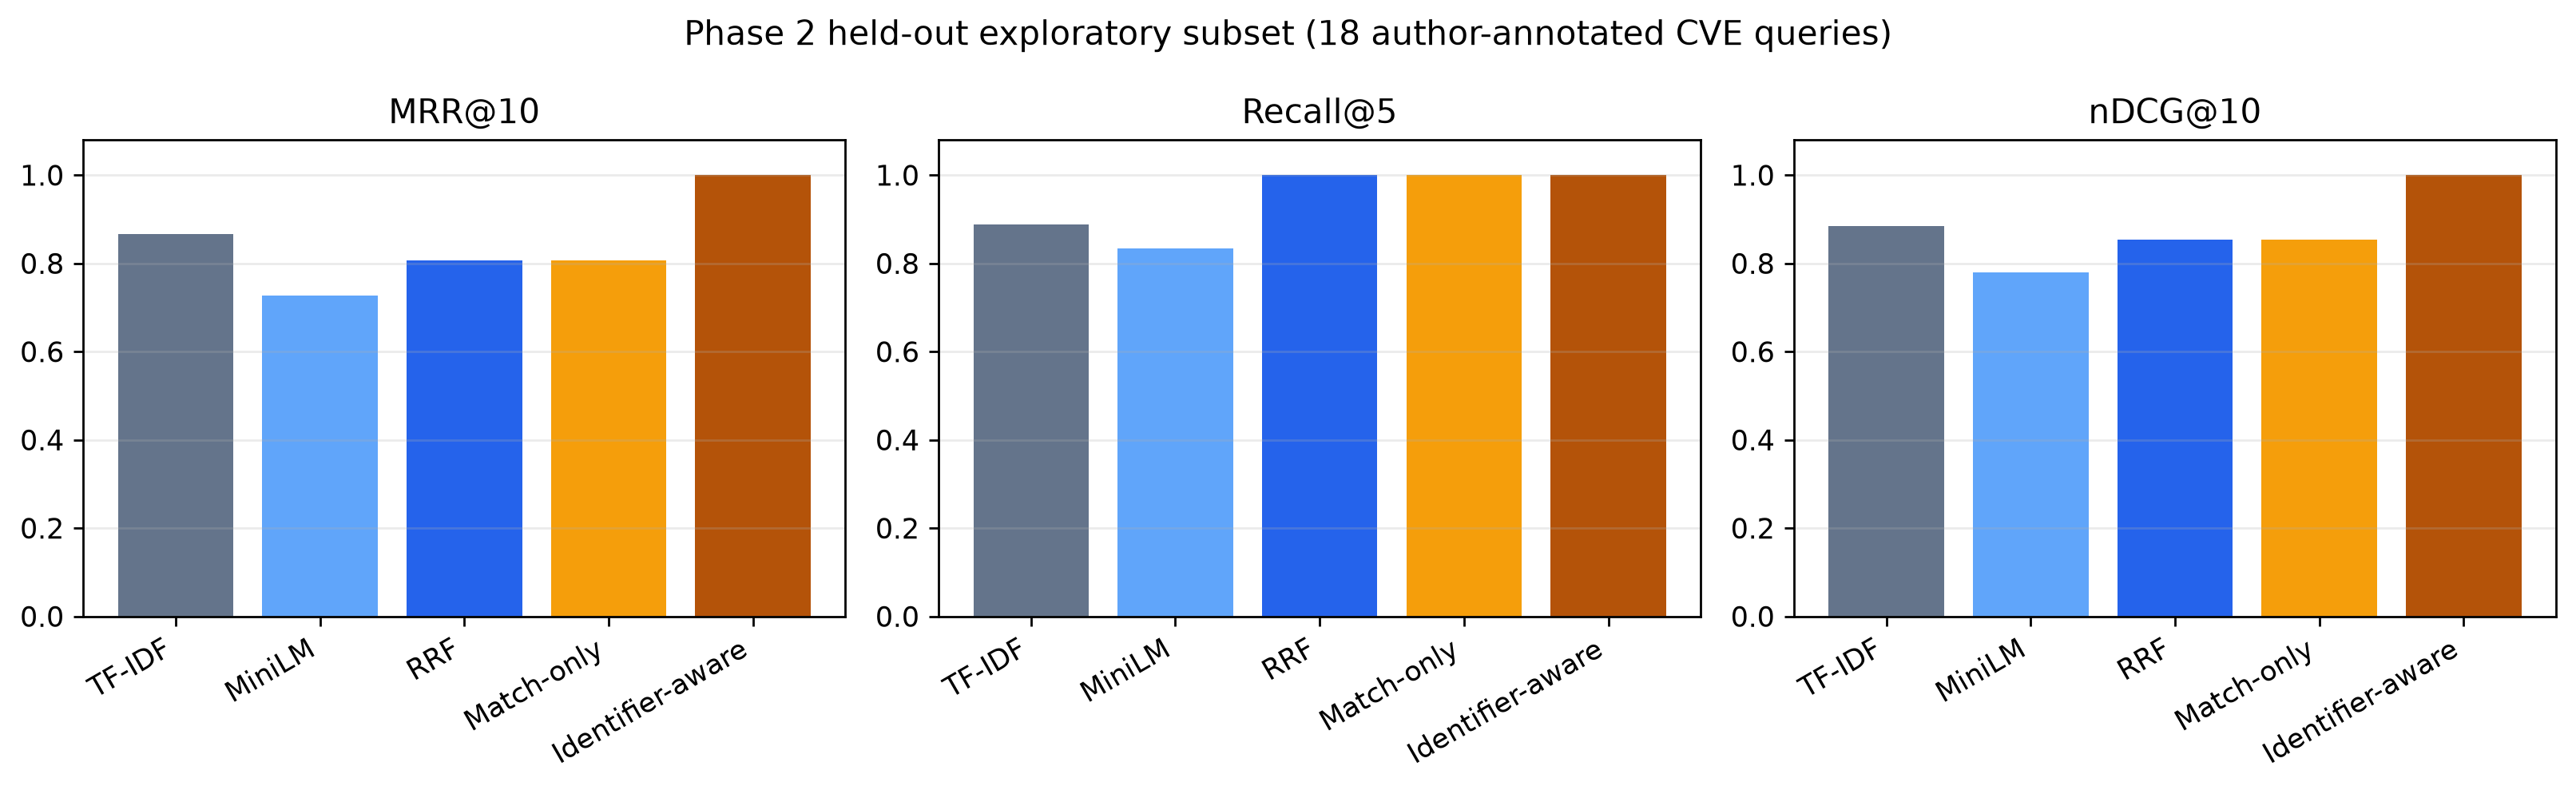
\includegraphics[width=\columnwidth]{../../outputs/phase2/stage18/figures/metric_comparison.png}
\caption{Held-out metrics from saved rankings.}\label{fig:metrics}
\end{figure}

\section{Ablation and Error Analysis}
Match-only equals RRF because the selected match weight is zero; the observed change comes from the conflict penalty. MiniLM is lower than RRF by .0796 with descriptive interval [-.1791, -.0009], while TF--IDF is higher by .0593 with interval [-.0333, .1704].

A concrete gain is cve-18, a query about CVE-2023-46747. RRF places its first known positive at rank 4, identifier-aware reranking places it at rank 1, and MiniLM places it at rank 21. No identifier-aware loss occurs in these 18 queries, so this paper does not invent an adverse example; the MiniLM case is an unsuccessful semantic-baseline retrieval example.
\begin{figure}[t]\centering
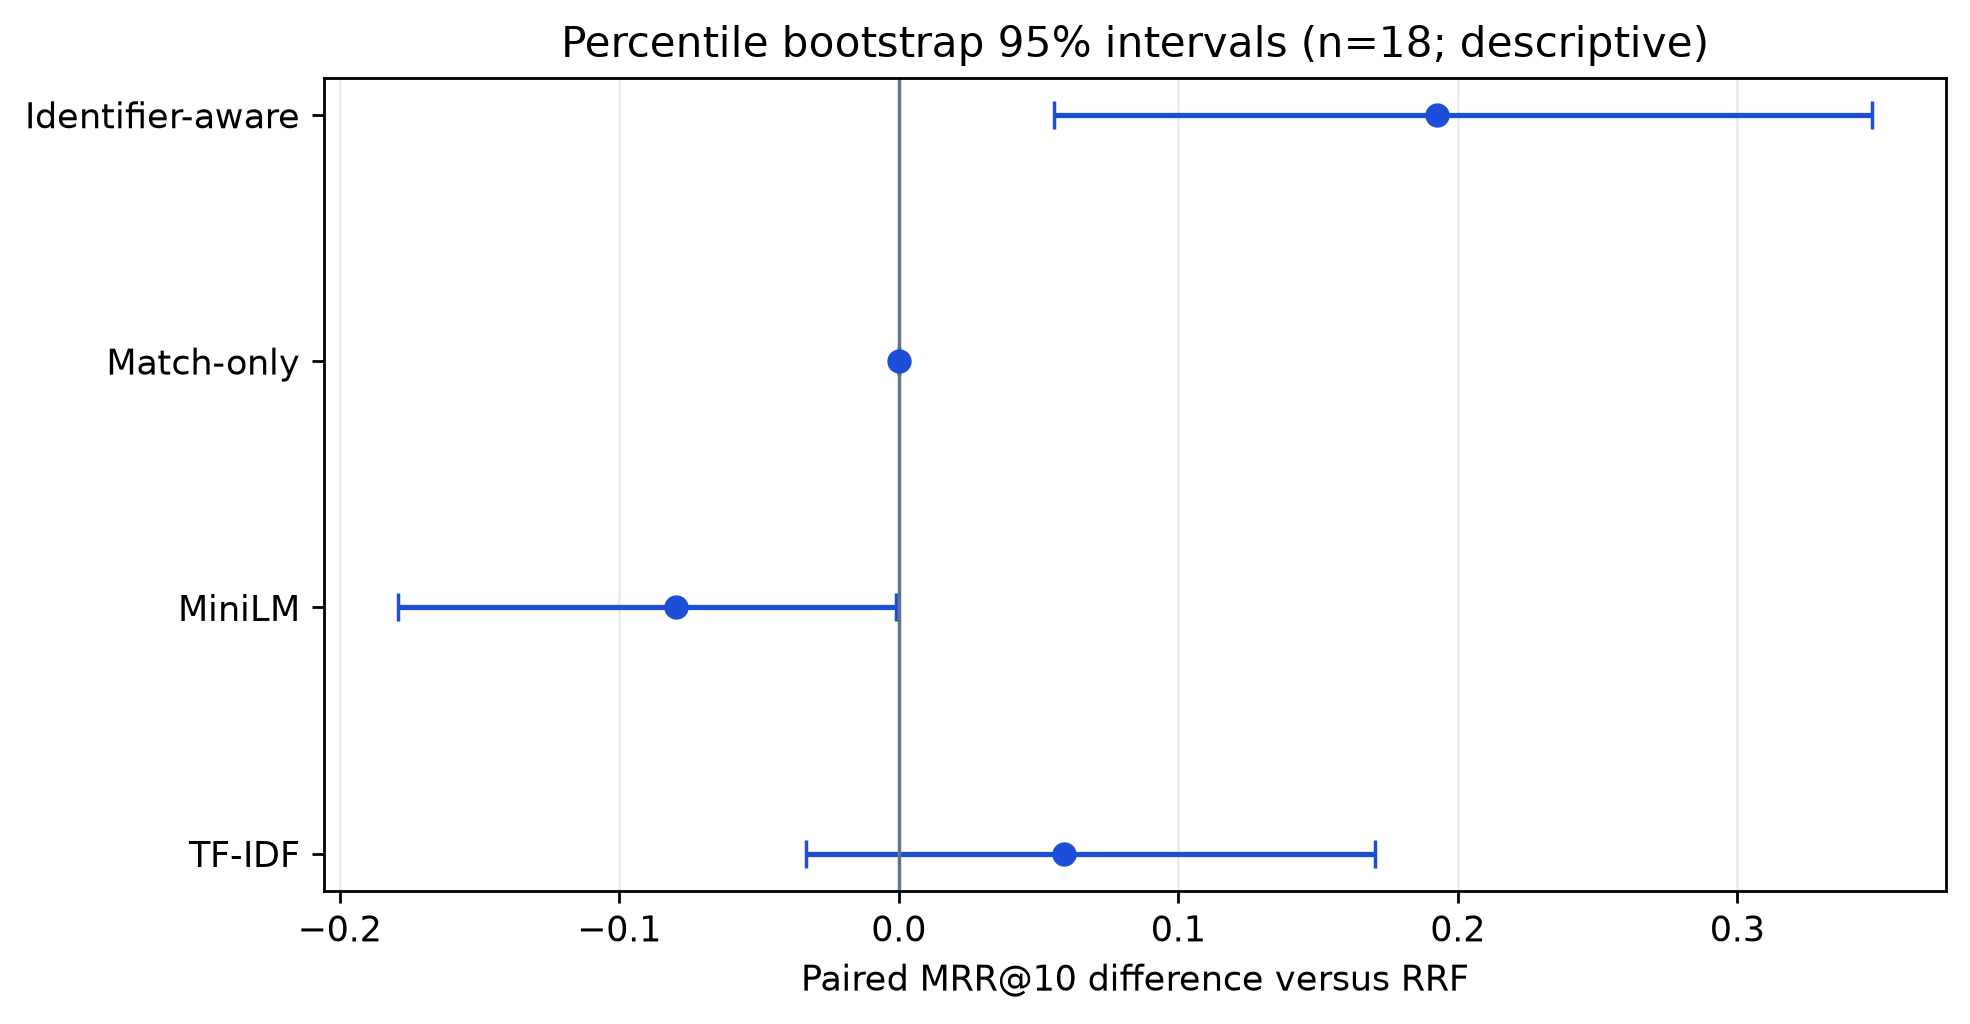
\includegraphics[width=\columnwidth]{../../outputs/phase2/stage18/figures/paired_mrr_differences.png}
\caption{Descriptive paired MRR differences versus RRF.}\label{fig:paired}
\end{figure}

\section{Computational Cost}
Median warm component times are 1.62 ms for TF--IDF, 21.12 ms for query embedding, .31 ms for dense ranking, .34 ms for RRF, and 21.80 ms for identifier reranking. Model load is 14.67 s and the embedding cache is a hit. These are sequential CPU components, not production end-to-end latency.
\begin{figure}[t]\centering
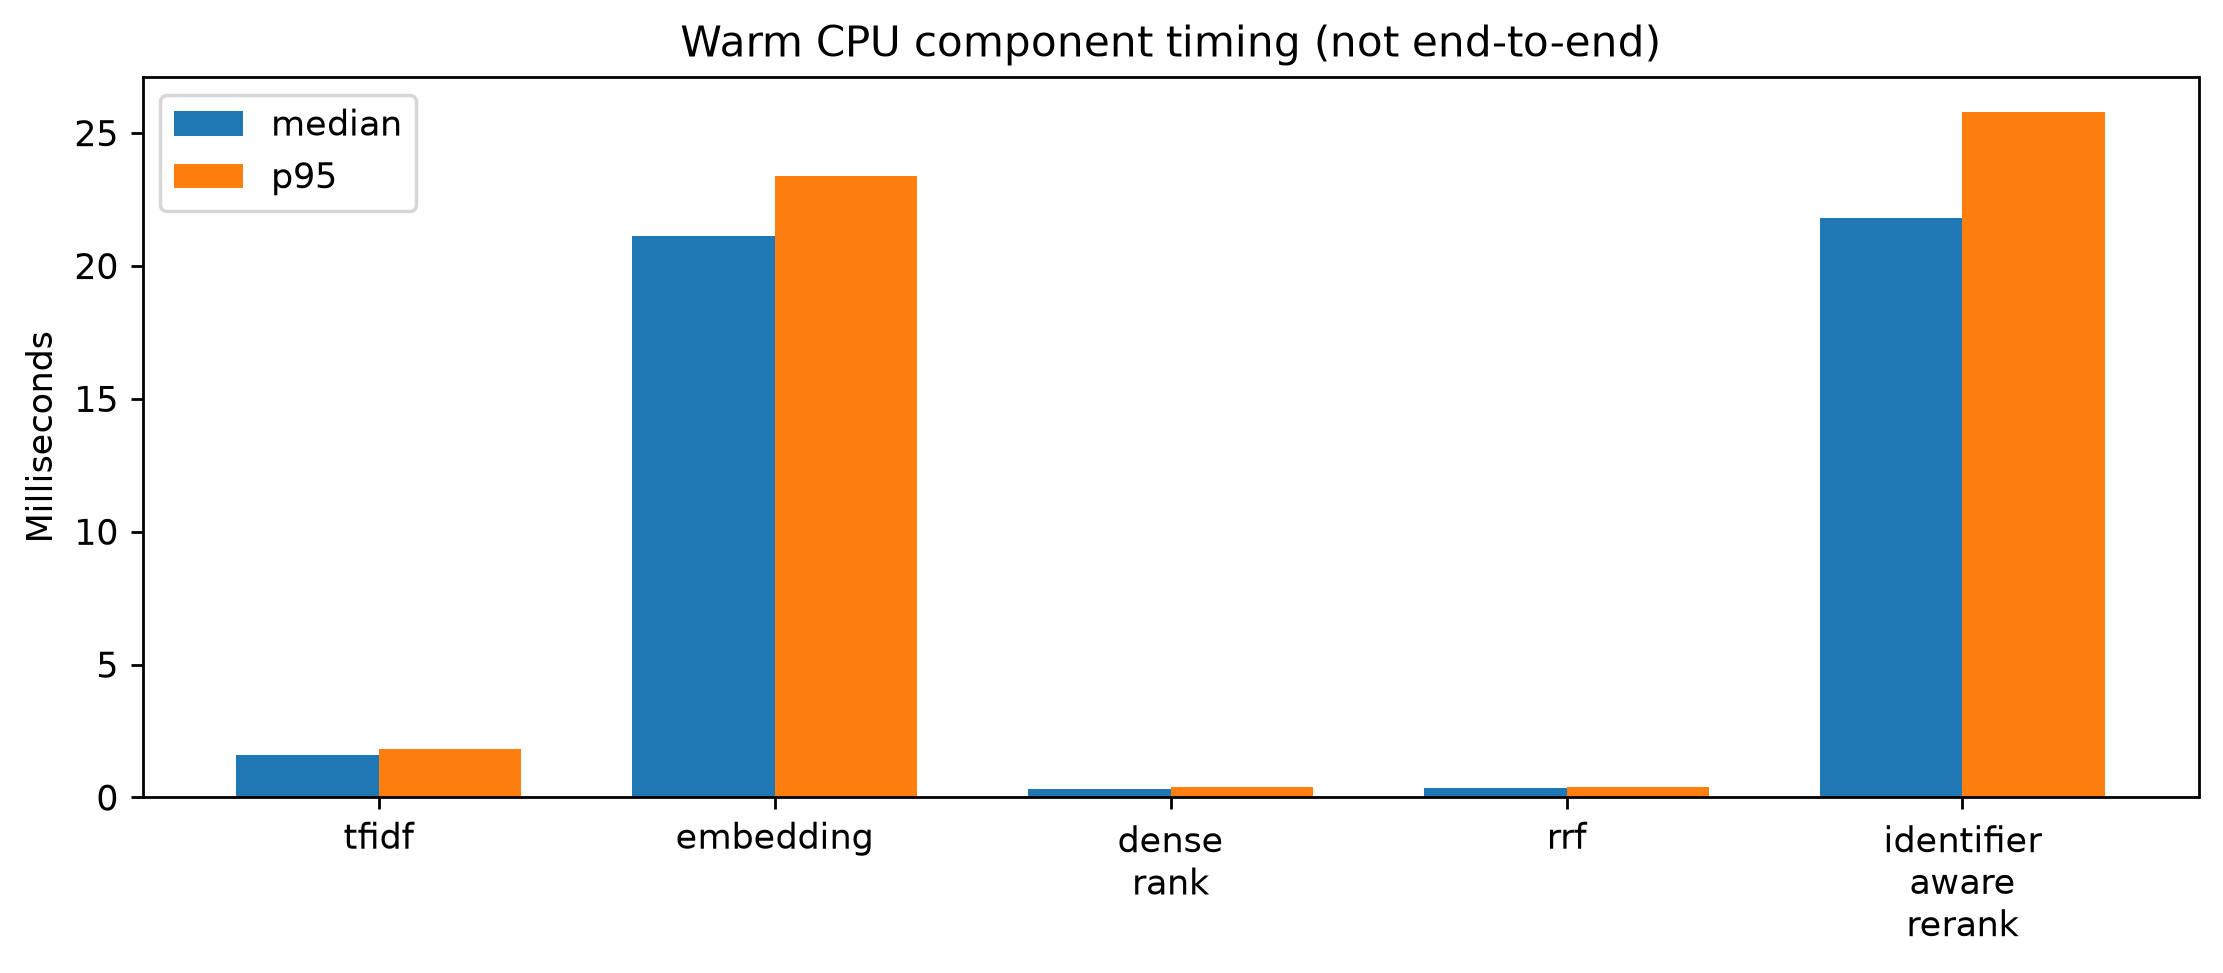
\includegraphics[width=\columnwidth]{../../outputs/phase2/stage18/figures/computational_cost.png}
\caption{Warm component timing.}\label{fig:cost}
\end{figure}
\section{Threats to Validity}
All labels originate with the project author; no independent agreement estimate exists. Candidate coverage is incomplete, only four explicit author negatives occur in eligible qrels, and 70 original author positives are unknown in derived qrels for lack of target evidence. The sample is small and CVE-only after answerability filtering. The held-out split limits direct tuning leakage but cannot remove construction bias or validate relevance. The parser covers explicit supported patterns, not aliases, typos, implicit references, or arbitrary identifier families. Bootstrap intervals over 18 author-annotated queries are descriptive rather than replication evidence.

\section{Conclusion}
This paper documents a reproducible exploratory evaluation of identifier-preserving hybrid retrieval. On a frozen author-annotated CVE subset, a selected conflict penalty improves observed rank-sensitive metrics over RRF while preserving Recall@5. Independent annotation, broader query families, complete pooling, and a new untouched test set are required before confirmatory conclusions.

\begin{thebibliography}{9}
\bibitem{reimers} N. Reimers and I. Gurevych, Sentence-BERT: Sentence Embeddings using Siamese BERT-Networks, in \emph{Proc. EMNLP}, 2019, doi: 10.18653/v1/D19-1410.
\bibitem{cormack} G. V. Cormack, C. L. A. Clarke, and S. Buettcher, Reciprocal rank fusion outperforms Condorcet and individual rank learning methods, in \emph{Proc. SIGIR}, 2009, doi: 10.1145/1571941.1572114.
\bibitem{luan} Y. Luan et al., Sparse, Dense, and Attentional Representations for Text Retrieval, \emph{TACL}, 2021, doi: 10.1162/tacl\_a\_00369.
\bibitem{gao} L. Gao, Z. Dai, and J. Callan, COIL: Revisit Exact Lexical Match in Information Retrieval with Contextualized Inverted List, in \emph{Proc. NAACL}, 2021, doi: 10.18653/v1/2021.naacl-main.241.
\bibitem{beir} N. Thakur et al., BEIR: A Heterogeneous Benchmark for Zero-shot Evaluation of Information Retrieval Models, in \emph{NeurIPS Datasets and Benchmarks}, 2021.
\end{thebibliography}
\end{document}
